\chapter{Theoretische Grundlagen}

\section{Gammaastronomie}
\label{sec:Gammaastronomie}

Im Universum gibt es zahlreiche Prozesse, bei denen hochenergetische Teilchen entstehen, oder auf diese Energien beschleunigt werden.
Bei diesen Teilchen handelt es sich zum großen Teil um Protonen oder leichten  Atomkernen bis hin zu Eisen, aber auch Elektronen oder Myonen
sind Bestandteil der Kosmischen Strahlung.
Ein großer Teil der Beschleunigung geschieht in Druckwellen, wie sie bei Sternexplosionen vorkommen und dabei spielt das Modell der
Fermi-Beschleunigung erster und zweiter Ordnung eine große Rolle.
%Bei der Fermi-Beschleunigung wird das Medium, indem die Druckwelle propagiert, durch ein Plasma beschrieben, welches Magnetfeldstörungen mit sich führt.
%Wenn ein geladenes Teilchen auf eine solche Störung, welche sich mit einer Geschwindigkeit $v$ durch das Medium bewegt, trifft, wird es durch die
%Lorentzkraft mit einem Winkel $\theta$ elastisch gestreut.
%Wenn nun alle möglichen Winkel berücksichtigt werden, ergibt sich eine Energiegewinn von
%\begin{equation*}
%  \left\langle \frac{\delta E}{E} \right\rangle = \frac{8}{2}\left(\frac{v}{c}\right)^2\text{ .}
%\end{equation*}
%Bei einer typischen Druckwellengeschwindigkeit von $v=\SI{e4}{\m\per\s}$\cite[14]{HESS} ergibt sich ein Energiegewinn von $\SI{4.5e-9}{\m\per\s}$.
%Dies wird Fermibeschleunigung zweiter Art genannt und kann die große Beschleunigung in Supernovae nicht alleine erklären.
%
%Ein größeren Beitrag liefert die Fermibeschleunigung erster Art, bei der die Teilchen durch mehrfaches durchqueren der Schockfront beschleunigt werden.
%Der Energiegewinn beträgt für alle Streuwinkel
%\begin{equation*}
%  \left\langle \frac{\delta E}{E} \right\rangle \approx \frac{2}{3}\frac{\delta v}{c} \text{ ,}
%\end{equation*}
%wobei $\delta v$ der Geschwindigkeitsunterschied zwischen der Materie hinter und vor der Schockwelle ist.

Für den Teilchenfluss der Kosmischen Strahlung direkt nach der Fermibeschleunigung in Schockfronten gilt
$\Phi(E)\approx E^{-2}$.
Wenn die Strahlung mit dem extragalaktische Plasma wechselwirkt, wird das Spektrum um $E^{-\frac{1}{3}}$ steiler und
da es auch das Plasma der Milchstraße durchqueren muss, damit es im Sonnensystem gemessen zu werden kann, wird
der Teilchenfluss der Kosmischen Strahlung durch $E^{-2.7}$\cite[5]{Cosmic_rays} beschrieben.

Jedoch erklären diese Prozesse nicht den gemessenen Energiefluss von ultra hochenergetischen Teilchen, denn bei Energien von $\SI{3e15}{\eV}$ tritt ein erstes
"knee" im Spektrum auf, welches nicht durch die Fermibeschleunigung erklärt wird.
Die Phänomene die Materie bis auf diese Energien beschleunigen, sind noch nicht vollständig erforscht.
Ein möglicher Prozess wäre die Beschleunigung durch elektrische Potentialunterschieden oder der Zerfall von Dunkler Materie speziell könnte
hochenergetische Teilchen erzeugen.

Diese hochenergetische Teilchenstrahlung erzeugt durch Wechselwirkungen oder Zerfälle Gammastrahlung.
Wichtige Prozesse bei der Erzeugung hochenergetischer Photonen sind die Wechselwirkungen von Photonen und Elektronen.
Die Prozesse, bei denen Gammastrahlung entsteht, sind die inverse Compton-Streuung, wobei das geladene Teilchen Energie auf das Photon
überträgt, die Annihilation, welche den Umkehrprozess der Paarerzeugung darstellt und aus einem Elekron Positron Paar
ein Photon erzeugt, und die Bremsstrahlung, wobei ein Photon bei der Impulsänderung gelandener Teilchen abgestrahlt wird.

\begin{figure}
  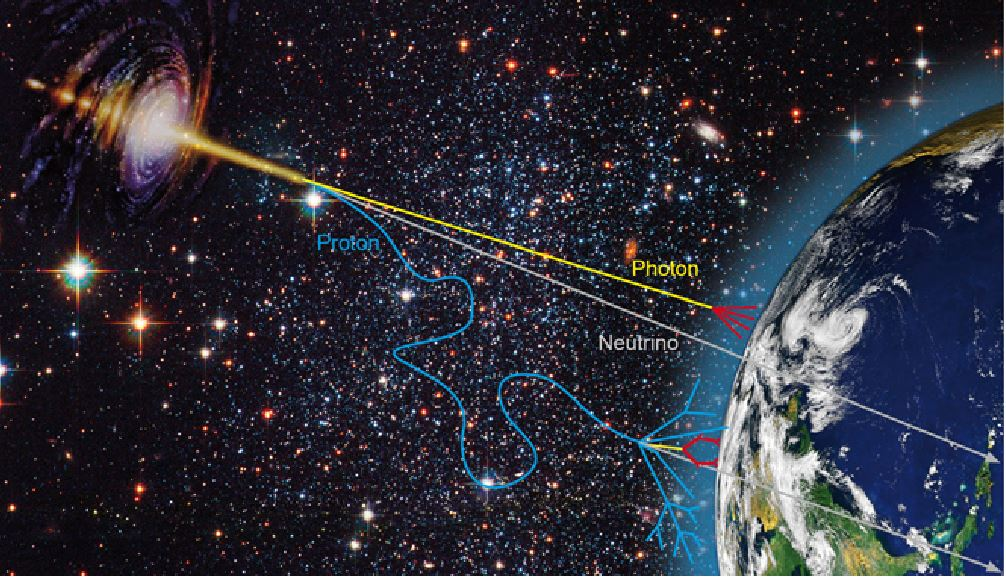
\includegraphics[width=0.7\textwidth]{Plots/Folie5.JPG}
  \centering
  \caption{Skizzierter Weg der Kosmischen Strahlung zur Erde. Die Gamma- und Neutrinostrahlung gelangt auf direktem Weg zur Erde, im Gegensatz
            zur geladenen Teilchenstrahlung, die durch kosmische Magnetfelder abgelengt werden. Die Gammstrahlung wird durch Gaswolken teilweise
            absorbiert. Die Neutrinostrahlung ist jedoch schwer zu detektieren.}
  \label{abb:Folie5}
\end{figure}

\autoref{abb:Folie5} stellt den Weg der Kosmischen Strahlung zur Erde dar, wobei die Photonen nicht mit kosmischen Magnetfeldern wechselwirken
und somit deren Ursprungsrichtung bekannt ist. Jedoch wechselwirken die Photonen mit interstellarem Staub, der zwischen der Erde und der
Quelle ist, wodurch ein Teil der Gammastrahlung nicht zur Erde gelangt.

Diese hochenergetischen Photonen oder auch Gammastrahlung genannt, können entweder direkt mithilfe von Satelliten im Weltraum oder indirekt über das in
der Atmosphäre entstehende Schauer mithilfe von Cherenkov Teleskopen auf der Erdoberfläche beobachtet werden.
Aufgrund der hohen Energien der Gammstrahlung können die Satelliten nur mithilfe von Szinillationszählern diese messe und nicht durch Spiegelteleskope,
da diese hohen Frequenzen nicht gespiegelt werden, sondern durch die Spiegeloberfläche transmittieren.
Diese energiereiche Strahlung sorgt jedoch dafür, dass in der Erdatmosphäre durch die Wechselwirkung mit den Luftmolekülen ein hochrelativistisches
Teilchenschauer ensteht, welches aus überlichtschnellen geladenen Teilchen bestehen.
Da sich bei Geschwindigkeiten über der Lichtgeschwindigkeit des Mediums die durch die Polarisierung entstandenen elektromagnetischen Wellen
nicht mehr destruktiv überlagern, entstehen Cherenkov-Blitze mit einer Dauer von $\SI{150}{\nano\s}$\cite{Cherenkov_Licht}, welche sich kegelförmig
mit einem spezifischen Winkel von
\begin{equation}
 cos(\theta) = \frac{1}{n\beta}
\end{equation}
ausbreitet und von den Cherenkov
Teleskopen am Boden beobachtet werden können.
Der Winkel $\theta$ hängt von dem Brechungsindex $n$ der Luft ab, welcher von der Feuchtigkeit und Dichte der Luft abhängt und somit höhenabhängig ist.
Das kontinuierliche Spektrum der Cherenkov-Strahlung besitzt eine zur Frequenz proportionale Intensität im sichtbaren Bereich und
wird daher als bläulich wahrgenommen.
Die Kamera des Teleskopes löst aus, wenn eine bestimmte Anzahl an Photonen des Schauers registriert wird und nimmt
für eine Dauer von $(150-300)\si{\nano\s}$ Bildmaterial auf.
Da sowohl hochenergetische Gammastrahlung als auch Teilchenstrahlung
Schauer in der Atmosphäre erzeugen, gibt es einen großen Untergrund, der separiert werden muss.

\section{Cherenkov Teleskope Array (CTA)}
\label{sec:CTA}

Das geplante Cherenkov Teleskop Array wird von einer internationalen Kollaboration von 210 Instituten aus 32 Ländern\cite{CTA_consortium} geführt
und bildet den nächste Schritt in der hochenergie Gammaastronomie.
Mit einer Gesamtanzahl von 108 Teleskopen hat das Array nach Simulationen zur Folge in seinem Hauptenergiebereich eine Sensitivität von $\SI{0.1}{\percent}$
des Energieflusses des Krebsnebels, wodurch es ungefähr zehn mal sensitiver wie das HESS-Experiment ist\cite{CTA_paper}.
Da der Teilchenfluss $\Phi$ der kosmischen Strahlung dem Potenzgesetz $\Phi \propto E^{-2.7}$\cite[5]{Cosmic_rays} folgt,
treffen bei einer Energie $E$ von $\SI{1}{\tera\eV}$ noch $\SI{1}{\per\m\squared\per\s}$ Teilchen auf die Erdatmosphäre.
Um dennoch genug Statistik zu besitzen, muss eine möglichst große Himmelfläche observiert werden.
CTA beobachtet durch die große Anzahl an Teleskopen, bei einer Beobachtungszeit von $\SI{0.5}{\hour}$, Photonen mit einer Energie von $\SI{1}{\tera\eV}$ auf einer
Fläche von $\SI{10e6}{\m\squared}$\cite{CTA_ob}.
Durch 3 verschiedene Teleskopgrößen, kann CTA Photonen mit Energien von $\SI{30}{\giga\eV}$ bis $\SI{300}{\tera\eV}$ detektieren.
Die Teleskop Arten bestehen aus dem LST (Large Sized Telescope) mit einer Spiegelgröße von $\SI{23}{\m}$, dem MST (Medium Sized Telescope)
mit einer Größe von $\SI{11.5}{\m}$ oder $\SI{9.7}{\m}$ und dem SST (Small-Sized Telescope), welches eine Größe von $\SI{4.3}{\m}$ oder $\SI{4.0}{\m}$
besitzt\cite{CTA_tec} .
Um die ganze Bandbreite der Beschleunigungsprozesse im Universum untersuchen zu können, wird eine solche Energiebreite benötigt.
Insbesondere kann das "knee" des Energiespektrums bei $\SI{3e15}{\eV}$ genauer untersucht werden.
Die hohe Sensitivität und die niedrige Energieuntergrenze ermöglichen die Entdeckung neuer Quellen mit einer starken Rotverschiebung, die nur bei niedrigen
Energien sichtbar sind, da die höher energetische Gammastrahlung mit der Hintergundstrahlung wechselgewirkt hat und somit nicht beobachtet werden kann.

\section{Maschinelles Lernen}
\label{sec:ML}

Aufgrund des geringen Teilchenfluss bei hohen Energien, muss die Anzahl an beobachteten Ereignissen bei modernen
Experimenten stark ansteigen, wodurch eine händische Analyse unmöglich wird.
Daher werden Algorithmen trainiert, die diese Aufgabe übernehmen.
Diese Algorithmen müssen jedoch intelligente Entscheidungen eigenständig treffen können, was künstliche Intelligenz
genannt wird.
Das maschinelle Lernen wird als Teilgebiet der künstlichen Intelligenz verstanden. Hierbei lernen Algorithmen aus Datensätzen,
indem sie verschiedene Optimierungsverfahren der Mathematik nutzen, um eine Fehlerfunktion zu minimieren.
Und ein trainierter Algorithmus trifft Vorhersagen für neue Datenpunkte.

Der Bereich des maschinellen Lernens wird in das überwachte Lernen, bei dem das Ergebnis und die Eingangsdaten bekannt
sind und das unüberwachte Lernen, bei dem der Algorithmus nur die Eingangsdaten kennt und in diesen Daten Muster sucht, gegliedert.
Zwei große Aufgabengebiete im Bereich des überwachten Lernens sind die Regression und die Klassifikation. Die Regression bildet
auf die reelen Zahlen ab und die Klassifikation auf $N$ Klassen.
Die Regression kann somit als Grenzfall $N \to \infty$ der Klassifikation verstanden werden.

Das Modell der Regressionsanalyse benutzt die abhängige Variable $y$ die über eine Funktion $f(X,\theta)$ von der Variable $X$ abhängt, um
den Parameter $\theta$ so zu optimieren, dass für $\hat{y} = f(X,\theta) + L(\hat{y},y)$ der Fehler
$L(\hat{y},y)$ minimiert wird.
Wenn $\vec{\theta}$ aus k Parametern besteht und $(X_i,y_i)$ $N$ Tupel sind, müssen drei Fälle unterschieden werden.
Im ersten Fall gilt $k>N$, was zu einem unterbestimmten System führt.
Für unterbestimmte Syteme gibt es nicht genug Datenpunkte, um alle Parameter vorherzusagen und viele Regressionsmethoden
führen zu keinem Ergebnis.
Bei $k = N$ existiert genug Information um ein lineares System exakt zu lösen.
Im letzten Fall gilt $k<N$, was das System überbestimmt werden lässt, wodurch es mehrere Lösungen gibt und
es wird die Lösung gewählt, die den Fehler minimiert.
Damit die Regressionsanalyse funktioniert, muss der Trainingsdatensatz das Problem vollständig repräsentieren. Außerdem darf der Fehler $L(\hat{y},y)$ keinen Trend
und keine Korrelation besitzen.
Eine weitere Annahmen über das Problem muss sein, dass das Problem eine unkorreliert und linear unabhängig Variable $X$ besitzt.
Wenn ein Problem eine unkonstante Varianz des Fehlers besitzt, muss dies durch eine gewichtete Methode korrigiert werden.

\section{Random Forest Regressor}
\label{sec:RF}

Eine Methode des überwachten Lernens, welche für die Regression verwendet werden kann, stellt der Random Forest Algorithmus dar. Dieser Algorithmus baut
einen Wald aus mehreren unkorrelierten Entscheidungsbäumen auf, die eigenständige Vorhersagen treffen, über die gemittelt wird.

Ein Entscheidungsbaum wird aufgebaut, indem der Datensatz in Teildatensätze aufgeteilt wird, wobei ein gewähltes Kriterium optimiert wird.
Dieses Kriterium
kann die Gini Unreinheit oder der Informationsgewinn sein, bei der Regression wird jedoch häufig die Varianz Reduktion verwendet.
Bei dieser Optimierung wird in jedem Schritt der mittlere quadratische Fehler
\begin{equation}
  H(X_m) = \frac{1}{N_m}\sum_{i\in N_m}(y_i-c_m)^2
\end{equation}
jedes Teildatensatzes $m$ minimiert, mit
\begin{equation}
  c_m = \frac{1}{N_m}\sum_{i\in N_m}y_i
\end{equation}
als Mittelwert der Vorhersage $y_i$ für jeden Datenpunkt $i$.
Dies wird rekursiv wiederholt und somit der Baum ausgebaut, bis der Algorithmus ein Abbruchkriterium erfüllt.
Dieses Abbruchkriterium kann eine vorher festgelegte maximale Tiefe
des Baumes sein, eine minimale Größe des Datensatzes, der getrennt werden soll, oder eine minimale Größe des getrennten Datensatzes. Nach Erreichen der Abbruchbedigung bildet
$c_m$ des letzten Schrittes die endgültige Vorhersage.

Bei Entscheidungsbäumen gibt es eine Vielzahl von Umsetzungen.
Die aktuellsten Arten sind jedoch der C5.0 und der CART Algorithmus\cite[1]{CART}.
Die Besonderheit am C5.0 Algorithmus bildet, im Gegensatz zum CART Algorithmus, die nicht notwendige binäre Trennung des Datensatzes,
jedoch kann mit ihm keine Regression durchgeführt werden.
Im \textsc{scikit-learn}-Framework\cite{scikit-learn} wird eine CART Implementierung des Entscheidungsbaums benutzt, welche zur
Regression genutzt werden kann und die Varianze Reduktion als Optimierungskriterium nutzt.

Die Vorteile eines Entscheidungsbaums sind die Interpretierbarkeit, der logarithmische Zusammenhang zwischen Trainingsdauer und Datengröße und die einfache Datenpräparation.
Außerdem besteht keine Anfälligkeit gegenüber unbedeutenen Attributen.
Jedoch besteht eine Gefahr des Übertrainierens, was bei einem zu großen Ausbauen des Baumes dazu fürht, dass der Trainingsdatensatz nachgebildet
wird und die Vorhersagen für einen unabhängigen Testdatensatz somit unpräzise werden.
Desweiteren kann es zu einer Verzerrung beim Vorhersagen kommen, wenn der Trainingsdatensatz eine Verzerrung aufweist.
Außerdem sind die Entscheidungsbäume nicht stabil gegenüber Änderungen im Datensatz, wwas zu einer hohen Varianz bei Vorhersagen
unterschiedlicher Bäume führt.
Da der Entscheidungsbaum zu den gierigen Algorithmen gehört, welche die Entscheidung aufgrund des derzeitig besten Gewinn treffen, findet dieses Verfahren sehr schnell ein
Optimum, jedoch bildet dieses Extremum nicht immer das globale Extremum und somit nicht die optimalste Lösung.
Die letzten beiden Nachteile können durch die Erweiterung des Entscheidungsbaum zu einem Entscheidungswald behoben werden.

Dieses Verfahren wird Random Forest(RF) genannt. Beim Random Forest werden eine Vielzahl von Entscheidungsbäume die, um Unkorreliertheit der Ergebnisse zu erreichen, mit
zufällig ausgewählten Teildatensätzen und Attribute trainiert werden. Das Ergebnis des RF ergibt sich durch eine Mittelung über alle Entscheidungsbäume.
Wenn die Anzahl der Entscheidungsbäume erhöht wird, konvergiert der generalisierte Fehler
\begin{equation}
  PE = P_{X,y}(mg(X,y)<0)
\end{equation}
gegen
\begin{equation}
  P_{X,y}(P_\theta(h(X,\theta)=y)-\max_{j\neq y}P_\theta(h(X,\theta)=j)<0)
\end{equation}
und es kann durch eine Vergrößerung des Waldes nicht zum Übertraining kommen\cite[7]{RandomForests_Breiman}. Bei diesem Theorem bildet
\begin{equation}
  mg(X,y) = av_k I(h_k(X)=y) - \max_{j \neq y}av_k I(h_k(X)=j)
\end{equation}
die Gewinn Funktion, $h_k(X)$ die Vorhersage der einzelnen Entscheidungsbäume und $I(\cdot)$ die charakteristische Funktion, welche eine $1$ ergibt, wenn der
Entscheidungsbaum das geforderte Ergebnis liefert und eine $0$ wenn nicht. Wenn die $mg(X,y) > 0$ gilt, sagt der Entscheidungsbaum das richtige Ergebnis vorher.

Um einen unkorrelierten Wald zu erhalten, muss die Auswahl der Teildatensätzen und der Attribute zufällig und unabhängig getroffen werden. Dazu kann unteranderem das Adaboost
Verfahren oder das Bagging verwendet werden. Das in \textsc{scikit-learn} verwendete Bagging funktioniert, indem aus dem Datensatz $N$ Stichproben der Größe
$M$ gezogen werden und für die $N$ Entscheidungsbäume verwendet werden. Die $N$ Ergebnisse werden am Ende gemittelt oder zusätzlich mit der Genauigkeit des jeweiligen Ergebnisses gewichtet.
Auch die Attribute werden in einem Umfang, der festgelegt werden kann, zufällig gezogen.
Hierdurch wird der Trend der einzelnen Ergebnisse größer, die Standardabweichung der Ergebnisses jedoch ungleich geringer,
was Verzerrung-Varainz-Dilemma genannt wird. Die Standardabweichung wird soweit minimiert, dass es zu keiner Überanzupassung kommt
und Verzerrung möglichst klein bleibt.

Durch Kreuzvalidierung kann das Modell auf Übertraining untersucht werden. Hierbei wird der Datensatz aufgeteilt, um
den Algorithmus mit einem Teil zu trainieren und mit dem anderen unabhängigen Teil zu testen.
Die in \textsc{scikit-learn} implementierte Methode stellt die einfache Kreuzvalidierung dar, bei der der Datensatz
in $k$ Teildatensätze geteilt wird und jeder dieser Datensätze als Validierungsdatensatz
verwendet wird und $k-1$ Datensätze zum Training dienen.

\section{Energie Rekonstruktion}

Um die in \autoref{sec:Gammaastronomie} erwähnten Bilder auszuwerten, muss zunächst die Kamera kalibriert werden, da die Funktionsweise der elektronischen
Komponenten stark von äußeren Bedingungen beeinflusst wird.
Der nächste Schritt stellt das Extrahieren der wichtigen Information aus dem Kamerabild in Form der Hillas-Parameter dar.
Dabei wird angenommen, dass die Kamera das Schauer als Ellipse sieht, wobei diese Ellipse eine Länge $L$ und Breite $w$ besitzt.
Weitere Parameter sind die $x$ und $y$ Koordinate des Ellipsenmittelpunkts, sowie dessen Polarkoordinaten $r$ und $\phi$ oder der Rotationswinkel $\psi$
der Ellipsenhauptachse, welcher relativ zur Verbindungslinie zwischen Ellipsenmittelpunkt und Kameramittelpunkt gemessen wird.
Die geometrischen Hillasparameter sind in \autoref{abb:Hillas} dargestellt.
\begin{figure}
  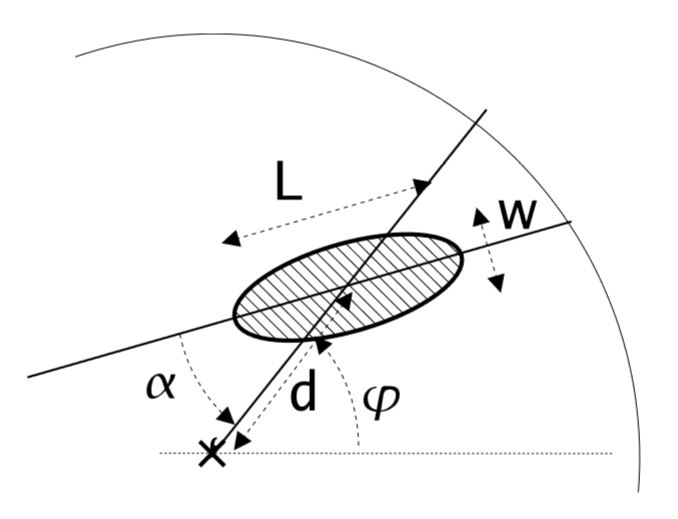
\includegraphics[width=0.7\textwidth]{Plots/Hillas.JPG}
  \centering
  \caption{Schematische Darstellung der Hillasparameter, die das Kamerabild des Schauers charakterisieren. Diese Parameter
            werden verwendet, um die Energie des primären Teilchens zu schätzen.}
  \label{abb:Hillas}
\end{figure}
Ein weiterer wichtiger Parameter bildet die totale Intensität des Bildes und da das CTA aus mehreren unterschiedlichen Teleskopen besteht, bekommt die Anzahl
der Teleskope, die das gleiche Schauer gesehen haben, und welche Art von Teleskope dieses Schauer gesehen hat, eine großer Bedeutung für die Anschließende
Signal Seperation und Energie Schätzung.

Diese Parameter werden genutzt um die Untergrundschauer von den Photon induzierten Schauern zu trennen.
Diese Aufgabe wird mit einer klassifizierungs Methode des maschinellen Lernens gelöst und der
Random Forest Klassifier stellt den qualifiziertesten Algorithmus dar.
Durch das Verhältnis von Signal zu Untergrund von $\frac{1}{1000}$\cite{Cherenkov_Licht} wird eine große Menge Trainingsdaten
benötigt, um eine gute Trennung zu ermöglichen.

Nach einer erfolgreichen Seperation können diese Parameter genutzt werden, um die Energie des Photons zu schätzen.
Dies kann durch Regressionsmethoden gelöst werde, wobei der Random Forest wieder den stablisten Algorithmus darstellt\cite{Cherenkov_Licht}.

Die in \autoref{sec:ML} aufgeführten Annahmen für eine erfolgreiche Regressionsanalyse, sind bei diesem Problem bestmöglich erfüllt. Die Trainingsdaten
werden durch Monte Carlo Simulationen erstellt, die die Wechselwirkung der primär und sekundär Teilchen mit der Atmosphäre und die Reaktion des Teleskopes
auf das Schauerlicht simuliert.
Dadurch repräsentiert der Trainingsdatensatz das Problem bestmögliche, jedoch wird der Fehler möglicherweise nicht durch eine Zufallszahl mit einem Mittelwert von $0$ dargestellt, da
mögliche systematische Fehler in der Simulation zu einer Verzerrung führen könnten.
Darüber hinaus werden die Parameter mit der größtmöglichen Präzession gemessen um den Fehler der Parameter zu minimieren,
jedoch sind aufgrund der Berechnung der Hillas Parameter, welche in [102]\cite{HESS}
genauer beschrieben wird, diese nicht linear unabhängig.
Auch die Varianz des Fehlers geht aufgrund der unterschiedlichen Sensitivitäten der Telescope nicht homogen
über den ganzen Energiebereich, was jedoch durch eine Gewichtung ausgeglichen werden könnte.

\section{Performance}

Um zu erkennen, ob das weiterentwickelte Modell eine genauere Vorhersage liefert als das Bisherige, muss die
Performance des Random Forests beurteilt werden können.
Ein mögliches Maß, um die Anpassungsgüte von Regressionsmodellen beurteilen zu können, stellt der Determinationskoeffizient dar, welcher
durch
\begin{equation}
  R^2 = 1 - \frac{\sum_i (y_i-\hat{y}_i)^2}{\sum_i (y_i - \overline{y})^2}
\end{equation}
definiert wird. Wobei $\hat{y_i}$ die Schätzwerte, $\overline{y}$ der Mittelwert und $y_i$ die Messwerte darstellen.
Der Determinationskoeffizient nimmt den Wert $1$ an, wenn das Modell die Messpunkte genau beschreibt. Wenn jedoch
$R^2 \leq 0$ kann das Modell als unbrauchbar eingestuft werden, da die Attribute $X$ keine Information zur
Lösung des Problems einbringen.

Dieser Koeffizient besitzt Grenzen der Interpretierbarkeit, da er nur eine Aussage über das gesamte Modell macht und
nicht über die Genauigkeit in einzelnen Wertebereichen.
Außerdem reagiert er empfindlich gegenüber Trends, die $R^2$ senken, obwohl das nicht bedeuten, dass das Modell die Abhängigkeiten des Problems
nicht gut beschreibt.
Desweiteren muss die gleiche Anzahl an Datenpunkten vorliegen, um Modelle
miteinander zu vergleichen.

Um einen ersten Überblick über die Genauigkeit des Algorithmus zu erhalten, wird die Wahrheit gegen die Vorhersage in einem
zwei dimensionalen Histogramm aufgetragen.
Dabei hat die Diagonale die Bedeutung der genauen Vorhersage und umso näher die gefüllten Container an dieser Geraden sind, umso besser
ist der Algorithmus.
Die Aussagekraft dieser Abbildung hängt von der Anzahl der Behälter ab und daher wird ein Raster von $300 \times 300$ verwendet.

Eine Aussage über die Genauigkeit des Algortihmus kann auch über den relativen Fehler getroffen werden. Dabei spielen der Mittelwert und der
Interquartile Abstand(IQA) von $\SI{68.26}{\percent}$, der durch
\begin{equation}
  IQA68 = Q84-Q16
\end{equation}
definiert wird, eine wichtige Rolle.
Dabei stellt $Q84$ das $\SI{84.13}{\percent}$ Quantil und $Q15$ das $\SI{15.87}{\percent}$ Quantil dar, welche durch die \textsc{numpy}-Bibliotheke
bestimmt werden, die das $q$-te Quartil als den $q \cdot N$-ten Wert eines geordneten Datensatzes der Größe $N$ definiert.
Der Mittelwert ist ein Maß für die Verzerrung und der IQA ist ein Maß für die Auflösung des Schätzers, wobei dies für unterschiedliche
Energie-Container untersucht wird, da aufgrund der energieabhängigen Statistik auch diese Werte über das Energiespektrum hinweg variieren.
